% Microelectronics Fabrication - Cheatsheet Spring 2015
% ======================================================================

% Dokumentklasse (Schriftgröße 6, DIN A4, Artikel)
\documentclass[6pt,letterpaper]{scrartcl}

% Seitenlayout und Ränder:
\usepackage{geometry}
\geometry{letterpaper,landscape, left=6mm,right=6mm, top=0mm, bottom=3mm,includeheadfoot} 

% Dokumentbeschreibung
\title{ECE571 MicroFab Cheatsheet Spring 2015}
\author{Yinglai Yang}

% Pakete laden
\usepackage[T1]{fontenc}
\usepackage[utf8x]{inputenc}	% Zeichenkodierung: UTF-8 (für Umlaute)   
\usepackage[english]{babel}		% Deutsche Sprache
\usepackage{multicol}			% Spaltenpaket
\usepackage{amsmath}			% Mathematische Formelzeichen
\usepackage{amssymb}			% Mathematische Formelzeichen
\usepackage{esint}				% erweiterte Integralsymbole
\usepackage{multicol}			% ermöglicht Seitenspalten  
\usepackage{booktabs}			% bessere Tabellenlinien
\usepackage{color}				% Farben
\usepackage{colortbl}			% für die Hintergrundfarbe einzelner Zellen in Tabellen
\usepackage{graphicx}			% Grafiken
\usepackage{pbox}				% Intelligent parbox: \pbox{maximum width}{blabalbalb \\ blabal}
%\usepackage{undertilde}			% Tilde unter Zeichen
\newcommand{\utilde}[1]{#1}
\usepackage{scrtime}			% Uhrzeit

%Farben
\definecolor{lightgray}{rgb}{0.8,0.8,0.8}
\definecolor{gray}{rgb}{0.9,0.9,0.9}

%Kopf- und Fußzeile

	
% Schriftart SANS für bessere Lesbarkeit bei kleiner Schrift
\renewcommand{\familydefault}{\sfdefault} 
\renewcommand{\emph}[1]{\textsf{\textbf{#1}}}

% Array- und Tabellenabstände vergrößern
\renewcommand{\arraystretch}{1.2}
\renewcommand{\vec}[1]{\ensuremath{\underline{\boldsymbol {#1}}}}


% Eigene Befehle
\newcommand{\todayV}{\the\day.\the\month.\the\year}                     	    	% Datum D.M.YYYY
\newcommand{\iset}[2]{\ensuremath{\bigl\{ \bigl. #1 \, \bigr| \, #2 \bigr\}}}		% intensional set
\newcommand{\eset}[1]{\ensuremath{\bigl\{#1\bigr\}}}								% extensional set
\newcommand{\norm}[1]{\ensuremath{\|#1\|}}											% Norm
\newcommand{\gk}[1]{\ensuremath{\left\lfloor#1\right\rfloor}} 						% Gaußklammer
\newcommand{\sprod}[2]{\ensuremath{\left\langle #1, #2 \right\rangle }}				% Skalarprodukt
\newcommand{\abs}[1]{\ensuremath{\left\vert#1\right\vert}} 							% Betrag
\newcommand{\mat}[1]{\ensuremath{\begin{bmatrix} #1 \end{bmatrix}}}					% Matrix
\newcommand{\vect}[1]{\ensuremath{\begin{pmatrix} #1 \end{pmatrix}}}				% Vektor
\newcommand{\mvect}[1]{\ensuremath{\left. \begin{matrix} #1 \end{matrix}  \right]}} % Matrixvektor
\newcommand{\ma}[1]{\ensuremath{\utilde{\bs {#1}}}}

% Abkürzungen
\newcommand{\ul}[1]{\ensuremath{\underline{#1}}}								%Untersteichen
\newcommand{\ol}[1]{\ensuremath{\overline{#1}}}									%Überstreichen
\newcommand{\Ra}[0]{\ensuremath{\Rightarrow}}									%Rightarrow
\newcommand{\ra}[0]{\ensuremath{\rightarrow}} 									%Rightarrow
\newcommand{\n}[0]{\ensuremath{\overline}}										%NOT
\newcommand{\bs}[1]{\ensuremath{\boldsymbol{#1}}}								%Fett und kursiv im mathmode
\newcommand{\diff}{\ensuremath{\ \mathrm d}}									%delta
\newcommand{\grad}{\ensuremath{\mathrm{grad}\ }}								%Gradient
\renewcommand{\div}{\ensuremath{\mathrm{div}\ }}								%Divergenz
\newcommand{\rot}{\ensuremath{\mathrm{rot}\ }}									%Rotation
\newcommand{\Sp}{\ensuremath{\mathrm{Sp}\ }}									%Spur
	% Für Mengen
	\newcommand{\N}{\ensuremath{\mathbb N}}
	\newcommand{\R}{\ensuremath{\mathbb R}}
	\newcommand{\C}{\ensuremath{\mathbb C}}

%Überschreibungen
\renewcommand{\arraystretch}{1.2}
\renewcommand{\vec}[1]{\ensuremath{\underline{\boldsymbol {#1}}}}


% ======================================================================
\newcommand\DOF{\mathit{DOF}}
\newcommand\NA{\mathit{NA}}
\newcommand\MTF{\mathit{MTF}}
\newcommand\CMTF{\mathit{CMTF}}
\newcommand\erfc{\mathrm{erfc}}
\newcommand\erf{\mathrm{erf}}

% Dokumentbeginn
% ======================================================================

\begin{document}


% Aufteilung in Spalten
\begin{multicols}{3}

% -------------------------------------------
% | 		Digitaltechik					|
% ~~~~~~~~~~~~~~~~~~~~~~~~~~~~~~~~~~~~~~~~~~~
%=======================================================================
\parbox{2.3cm}{
	
\includegraphics[width=2cm]{./img/UMASS.eps}
}
\parbox{4cm}{
	\emph{\huge{ECE571 MicroFab}}
}










\begin{center}
	Yinglai Yang, March 2015
\end{center}
% ======================================================================
\section{Miscellaneous}

\begin{tabular}{ r | l }
Si atom density & $5\times 10^{22} \mathrm{cm}^{-3}$ \\
Boltzmann constant & $\kappa_B = 8.62\times 10^{-5} \mathrm{eV/K}$ \\
Vacuum permittivity & $\epsilon_0 = 8.854\times 10^{-12} \mathrm{F/m}$ \\
$°C \rightarrow °K$ & $+273°$ \\
Capacity & $C = \frac{\epsilon_r \epsilon_0 A}{d}$ \\
Diffusivity & $D = D_0 \cdot \exp(-E_a/k_B T)$
\end{tabular}

% ======================================================================
\section{Ingot}

\subsection{Czochralski}
Crystalgrowth process:
\begin{enumerate}
	\item Polyxtals melted in a Qz crucible (>1500°C)
	\item Seedxtal put in contact with surface (seed determines orientation)
	\item Si atoms nucleate; ingot grows while being pulled up out of melt
\end{enumerate}

\subsection{Ingot Dopant Profile}
\textbf{Czochralski - CZ} \\
Segregation coefficient $k_0 = \frac{C_s}{C_l}$ \textit{(solid side / liquid side concentration)} \\
Dopant concentration profile: \framebox{$C_s(x) = C_0 k_0 (1-x)^{k_0 - 1}$} \\
Higher $k_0 < 1$ are often preferable $\leadsto$ flatter profile = more wafers with uniform dopant concentration \\
\\
\textbf{Floating Zone - FZ} \\
A ring heats up a small section of ingot and goes through ingot in \textbf{one} direction. Impurities move towards current liquid section. Used to clean ingot of impurities if a high $\rho$ ingot is wanted. Process drives impurities to one end of ingot. Repeat process to get better results.\\
Dopant concentration profile: \framebox{$C_s(x) = C_0 [1 - (1-k_0) exp(-\frac{-k_0 x}{L})]$}

% ======================================================================
\section{Wafer}
Crystal Orientation and Flats \\
TODO better image with same orientations as in lecture
%\begin{center}
%	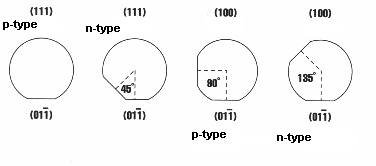
\includegraphics[width=6cm]{./img/wafer/flats.png}
%\end{center}


\subsection{Electrical Characterization}
\textbf{Dopant type} -- Dopant type of wafer can be determined using a \textbf{hot probe}. This is a setup with two connected probes on surface of wafer. One probe is heated and drives majority carriers away of itself. Direction of the resulting current tells the carrier type ($e^-$ or hole). \\
\\
\textbf{Impurity concentration} -- Impurity concentration can be inferred from resistivity. Use \textbf{four-point-probe} to measure resistivity. Outer probes enforce I, inner probes measure V. This setup prevents contanct resitance to distort result (contact resitance only at outer probes).
\begin{center}
	\parbox{3cm}{
		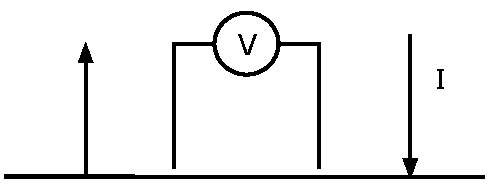
\includegraphics[height=1cm]{./img/wafer/four-point-probe.pdf}
	}
	\parbox{1cm}{
		$R=\frac{V}{I}$
	}
\end{center}

% ======================================================================
\section{Silicon Oxide}
\subsection{Oxide Growth -- Deal-Grove Model}
Oxide thickness \framebox{$d_{ox} = \frac{A}{2} \left(\sqrt{1+\frac{t+\tau}{A^2/4B}} - 1\right)$} \\ $\tau = \frac{d_i^2 + A d_i}{B}$; $d_i$ is initial thickness \\
\\
\vspace{0.2cm}
\textbf{Standard Simplifications}
\vspace{-0.4cm}
\begin{enumerate}
	\item $t \gg A^2/4B \leadsto$ "Thicker" oxides (parabolic growth): \framebox{$d_{ox} = \sqrt{B t}$}
	\item \vspace{-0.1cm} $t+\tau \ll A^2/4B \leadsto$ "Thinner" oxides (linear growth): \framebox{$d_{ox} = \frac{B}{A}(t+\tau)$}
\end{enumerate}
Also, note $\left( \frac{B}{A} \right)_{(111)} = 1.68 \left( \frac{B}{A} \right)_{(100)}$

\subsection{Oxide to Silicon Relationship}
A unit cube of Si will become $SiO_2$ with a volume that is 2.24 times bigger. If the growth is constrained to one dimension, this is the relationship of thickness.

Using this relationship: Of 100% silicon oxide, 45% will be under the original surface (45% silicon consumed to give 100% oxide).

\subsection{Electrical Characterization of Oxide}
\textbf{C-V profile} -- The capacity of the wafer can be measured. When the MOS structure is in \textbf{accumulation} or \textbf{inversion at low frequency}, the measured capacity $C = C_{ox}$. For \textbf{depletion} or \textbf{inversion at high frequency}, the measured capacity is smaller (capacitances in series).

To measure the capacity, a small alternating voltage is added to the DC voltage at the wafer. The resulting current will have a part that is phase-shifted compared to the voltage ($+90°$ or $+\pi/2 leadsto$ current precedes voltage).

Calculate C using $i(t) = C \frac{dv(t)}{dt}$

\subsection{High-k Dielectric Materials}
Recall $C = \frac{\epsilon A}{d}$. "High k" materials with $\epsilon_r$ greater than SiOx allow to get the same electrical behavior (capacity C) for the gate oxide with \textbf{thicker} spacing. \textbf{More space between channel and gate electrode} $\leadsto$ \textbf{smaller leakage current!}

% ======================================================================
\section{Lithography}
\subsection{System Parameters}
Rayleigh criterion/limit $R = \frac{1.22 \lambda}{d} f$; $d$: \textit{aperture diameter} \\
$\leadsto$ for lithography, \textbf{resolution} \framebox{$R = W_{min} = k_1 \frac{\lambda}{\NA}$}; $k_1$: \textit{process parameter} \\
\\
\textbf{Numerical aperture} \framebox{$\NA = n \cdot \sin (\alpha)$}; $n$: \textit{refractive index of medium between objective - wafer}; $\alpha$: \textit{objective lens acceptance angle} \\
\\
\textbf{Depth of focus (DOF)} \framebox{$\DOF = \frac{n \lambda}{\NA^2}$} \\
\\
\textbf{Modulation transfer function (MTF)} \framebox{$\MTF = \frac{I_{max} - I_{min}}{I_{max} + I_{min}}$} \\
\\
\textbf{Strive for:} $R \downarrow, \DOF \uparrow, \MTF \rightarrow 1$

\subsection{Photoresist}
\textbf{Contrast} \framebox{$\gamma = \frac{1}{\log(D_{100}/D_0)}$} \\
\textbf{Critical modulation transfer function (CMTF)} \framebox{$\CMTF = \frac{D_{100} - D_0}{D_{100} + D_0} = \frac{ 10^{-\gamma} - 1 }{ 10^{-\gamma} + 1 }$} \\
\\
$CMTF < MTF$ must hold for the image to resolve!

\subsection{Improving Resolution}
Methods without reducing $\lambda$:
\begin{itemize}
	\item \textbf{Immersion lithography} -- Add a liquid (DI water) between lens and PR $\leadsto \NA \uparrow$
	\item \textbf{Off-axis illumination}
	\item \textbf{Phase shift mask}
	\item \textbf{Optical proximity correction}
	\item \textbf{Double/multi patterning}
\end{itemize}
Reducing $\lambda$:
\begin{itemize}
	\item \textbf{Extreme ultraviolet (EUV)} -- $\lambda = 13\mathrm{nm}$ or lower. At these wavelengths there is no material that can act as a lens (it will all be absorbed). System of mirrors used instead (compare to astronomy).
	\item \textbf{X-ray}
\end{itemize}
Alternative: \textbf{Nano imprint lithography} uses a mold to print pattern into resist.
% ======================================================================
\section{Doping}
\subsection{Thermal Diffusion}
Typically, source on wafer surface. Drive-in by thermal diffusion. Two different cases:\\
\\
\textbf{Unlimited/constant source, predeposition} -- Dopant concentration at wafer surface held constant over whole diffusion process (normally \textbf{solid solubility!}). \\
$C(z,t) = C_S \erfc \left( \frac{z}{2\sqrt{Dt}} \right)$ \\
$Q_T(t) = \frac{2}{\pi} C(0,t) \sqrt{Dt}$ \\
$x_j = 2\sqrt{Dt} \erfc^{-1} \left( \frac{C_S}{C_B} \right)$ \\
\\
\textbf{Limited source, drive-in} -- A fixed amount of dopant $Q_T$ is applied to wafer surface. Amount given as surface concentration ($\mathrm{cm}^{-2}$). \\
$C(z,t) = \frac{Q_T}{\sqrt{\pi Dt}} \mathrm{e}^{-z^2/4Dt}$ \\
$x_j = \sqrt{4Dt \ln \left( \frac{Q_T}{C_B \sqrt{\pi Dt}} \right) }$ \\
\\
\textit{A case that often appears is a predeposition step followed by drive-ins (normally parasitic thermal processes). If $\sqrt{Dt_predep} \ll \sqrt{Dt_drive-in}$, then the dose is given by the predeposition, while the resulting concentration profile and junction depth can be approximated using the drive-in model.}\\
\textit{To combine multiple diffusion steps in a sequence use the sum of all $Dt$'s: $Dt_{eff} = Dt_1 + Dt_2 + \dots$}

\subsection{Ion Implantation}
\textbf{Impurity concentration} \framebox{$N(x) = N_p \mathrm{e}^{-(x-R_p)^2/2 \Delta R_p^2}$} \\
$R_p$: projected range \\
$\Delta R_p$: projected straggle \\
For implant completely in silicon \framebox{ $Q = \sqrt{2\pi} N_p \Delta R_p$ } \\
Junction depth \framebox{ $x_j = R_p \pm \Delta R_p \sqrt{2 \ln (N_p/N_B)}$ }







\end{multicols}


% Dokumentende
% ======================================================================
\end{document}
